\documentclass[11pt,english]{article}
\usepackage[T1]{fontenc}
\usepackage[utf8]{inputenc}
\usepackage[english]{babel}
\usepackage[pdfauthor={Lars Maiwald, Kevin Siebert}]{hyperref}
\usepackage{amsthm}
\usepackage{amssymb}
\usepackage{amsmath}
\usepackage{mathtools}
\usepackage{comment}
\usepackage{pdfpages}
\usepackage{fancyhdr}
\usepackage[headheight=14pt]{geometry}
\usepackage{graphicx}
\usepackage{caption}
\usepackage{subcaption}
\usepackage{siunitx}
\usepackage{csquotes}
\usepackage{hyphenat}
\usepackage{float}
\usepackage{xcolor}
\usepackage{cleveref}
\usepackage{listings}
\usepackage[lighttt]{lmodern}
\usepackage{appendix}
\usepackage{booktabs}
\usepackage[affil-it]{authblk}
\usepackage[backend=biber,style=phys,biblabel=brackets,pageranges=false,sorting=nyt]{biblatex}
\usepackage{multicol}
\usepackage{watermark}
%\addbibresource{}

\lstdefinestyle{CppStyle}{
  language=C++,
  stepnumber=1,
  numbersep=10pt,
  tabsize=4,
  showspaces=false,
  showstringspaces=false
}
\lstdefinestyle{PseudoStyle}{
  basicstyle=\small\ttfamily,
  stepnumber=1,
  numbersep=10pt,
  tabsize=4,
  showspaces=false,
  showstringspaces=false,
  keywordstyle=\color{black}\bfseries\em,
  keywords={,input, output, return, datatype, function, in, if, else, foreach, while, begin, end, }
}
\lstset{basicstyle=\small\ttfamily, style=CppStyle}

\crefname{equation}{}{}
\Crefname{equation}{\text{Equation}}{\text{Equations}}
% \crefname{section}{\text{Kapitel}}{\text{Kapitel}}
% \Crefname{section}{\text{Kapitel}}{\text{Kapitel}}
% \crefname{table}{\text{Tab.}}{\text{Tab.}}
% \Crefname{table}{\text{Tabelle}}{\text{Tabellen}}
% \crefname{figure}{\text{Abb.}}{\text{Abb.}}
% \Crefname{figure}{\text{Abbildung}}{\text{Abbildungen}}

\numberwithin{equation}{section}

%\hyphenation{Mathe-matik wieder-gewinnen}

\sisetup{
locale = DE,
range-phrase = \ldots,
separate-uncertainty=true,
scientific-notation=true,
}

\geometry{
  a4paper,
  left=2.5cm,
  right=2.5cm,
  top=3cm,
  bottom=3cm
}

\renewcommand{\footrulewidth}{0.4pt}
\renewcommand{\headrulewidth}{0.4pt}
\pagestyle{fancy}
\fancyhf{}
\rhead{Maiwald, Siebert}
%\lfoot{}
\lhead{\slshape\nouppercase{\leftmark}}
\cfoot{\thepage}
%\pagestyle{empty}

\hypersetup{
    colorlinks=true,
    linkcolor=blue,
    filecolor=magenta,      
    urlcolor=magenta,
    citecolor=green,
}
\urlstyle{same}

\graphicspath{ {resources/figures/} }

\allowdisplaybreaks

% \setlength\parindent{0pt}

%Einige nützliche Definitionen
\newcommand{\deriv}[2]{\frac{\mathrm{d} #1}{\mathrm{d} #2}}
\newcommand{\pderiv}[2]{\frac{\partial #1}{\partial #2}}
% \newcommand{\kommut}[2]{\left[ #1, #2 \right]}
% \newcommand{\tagthis}[1]{\addtocounter{equation}{1}\tag{\theequation}\label{#1}}
% \newcommand{\tagit}{\addtocounter{equation}{1}\tag{\theequation}}
% \DeclarePairedDelimiter\bra{\langle}{\rvert}
% \DeclarePairedDelimiter\ket{\lvert}{\rangle}
% \DeclarePairedDelimiterX\braket[2]{\langle}{\rangle}{#1 \delimsize\vert #2}
% \DeclarePairedDelimiterX\expval[2]{\langle}{\rangle}{#2 \delimsize\vert #1 \delimsize\vert#2}
% \DeclarePairedDelimiterX\matrixel[3]{\langle}{\rangle}{#1 \delimsize\vert #2 \delimsize\vert#3}
% \DeclarePairedDelimiterX\expv[1]{\langle}{\rangle}{#1}

\newcommand{\ie}{\textit{i.e.} }
\newcommand{\eg}{\textit{e.g.} }

\lstset{
	escapeinside={/*@}{@*/}, language=C++,
	basicstyle=\fontsize{8.5}{12}\selectfont,
	numbers=left,numbersep=2pt,xleftmargin=2pt,frame=tb,
    columns=fullflexible,showstringspaces=false,tabsize=4,
    keepspaces=true,showtabs=false,showspaces=false,
    backgroundcolor=\color{white}, morekeywords={inline,public,
    class,private,protected,struct},captionpos=t,lineskip=-0.4em,
	aboveskip=10pt, extendedchars=true, breaklines=true,
	prebreak = \raisebox{0ex}[0ex][0ex]{\ensuremath{\hookleftarrow}},
	keywordstyle=\color[rgb]{0,0,1},
	commentstyle=\color[rgb]{0.133,0.545,0.133},
	stringstyle=\color[rgb]{0.627,0.126,0.941}
}

\graphicspath{{./resources/images/}}

\thiswatermark{\centering \put(326.5,-68.0){\includegraphics[scale=1.2]{sciences_en.png}}}

\usepackage{abstract}
\newcommand{\myabstract}[1]{
\twocolumn[
  \maketitle             % full width title
  \begin{onecolabstract} % ditto abstract
    {#1}
  \end{onecolabstract}
\vspace{\baselineskip}
]}
\usepackage[backend=biber, style=phys]{biblatex}
\addbibresource{resources/references.bib}

\title{\textbf{Report: \\ Deep learning final project (miniprojects)}}
\author{Kevin Siebert%
	\thanks{\textsc{}s{\href{mailto:Kevin.Siebert@etu.unige.ch}{Kevin.Siebert@etu.unige.ch}}}}
\affil{Department of Informatics, Faculty of Science, \\ University of Geneva}
\date{Dated: \today}

\begin{document}
	\maketitle
	\vspace{-20pt}
	\begin{abstract}
		This is a report on the solution of the two mini projects proposed as a final project for the course Deep Learning (14X050). The solutions consists of this report and a GitHub archive containing the corresponding code (\thanks{\href{https://github.com/I-am-Rudi/DL_FinalProject}{Github Archive}}).
	\end{abstract}
	
	\section{Project} \label{sec:Proj1}
	\vspace{-10pt}
	\subsection{Introduction}
	The main goal of the first project is to compare the performance of basic neural network architectures. This is done with respect to a specific classification task where the network is supposed to predict the relationship (smaller or equal / larger) between two numbers of the MNIST dataset. A small selection from this dataset can be seen in \cref{fig:ex_pair}.
	
	\begin{figure}[H]
		\centering
		\includegraphics[width = .30\textwidth]{pair_example.png}
		\caption{Small selection of inputs from the dataset where every row represents on input and the caption show the corresponding target classes.}
		\label{fig:ex_pair}
	\end{figure} 


	\subsection{Architectures}
	For the structure of the networks, four variable architectures where chosen. For all architectures there is one one version which starts with several convolutional and Batchnorm layers and is followed by linear layers, another which is fully convolutional and every architecture has the possibility to switch between several or one output neuron depending on whether one hot encoded labels are used. 
	
	The fully convolutional networks are created on the basis of the mixed networks at initialization through the function \lstinline|convolutionize| which is based on the \lstinline|convolutionize| function \cite{Fleuret2022} defined in the lectures. They are not transformed after training but at initialization so they are trained as fully convolutional networks.
	
	One hot encoding is specified through the variable \lstinline|one_hot_encoding| at initialization and is enabled for all additional functions by the same variable.
	
	All architectures use ReLU as their internal activation functions and Sigmoid as their output activation. All models are initialized with 64, 64 and 32 for the number of neurons in the main branch for the hidden Linear layers.
	
	The first implemented architecture can be seen in \cref{fig:sn} it represents the ``naive'' approach where the images are passed through separate convolutional layers to extract their feature. The results are concatenated flattened and passed through fully connected linear layers/convolutional layers for the actual classification. This architecture will be called ``simple network'' (SN) from now on.
	
	\begin{figure}[H]
		\centering
		\includegraphics[width = .75\textwidth]{Simple_network.png}
		\caption{Diagrammatic visualization of the architecture for the simple network. (figure made using Inkscape)}
		\label{fig:sn}
	\end{figure}

	Of course an architecture like \cref{fig:sn} wastes some learning potential by separating the feature extraction. Therefore an attempt on improvement is made through the architecture in \cref{fig:ws} from now on called ``weight sharing network'' (WSN). Here, we do the feature extraction by passing Number 1 as well as Number 2 (one after the other) threw the first two convolutional layers, then concatenate and continue.
	
	\begin{figure}[H]
		\centering
		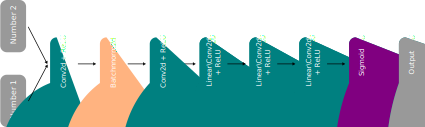
\includegraphics[width = .75\textwidth]{Weight_sharing_network.png}
		\caption{Diagrammatic visualization of the architecture for the weight sharing network.(figure made using Inkscape)}
		\label{fig:ws}
	\end{figure}

	The following two architectures rely on the concept of auxiliary classifiers as described in \cite{Szegedy2014}. The basic idea is to branch of the main architecture at some point to do the same or another classification task from the input. This part is also trained and the loss is added (usually multiplied by a some fraction smaller than one) to the loss of the main branch. This part is usually discarded when evaluating the model.
	
	\Cref{fig:saux} takes the most simple approach to this concept by branching of and trying to perform the same classification as the main branch and will therefore be called ``Simple auxiliary classifier model'' (SAUX) from now on.
	
	\begin{figure}[H]
		\centering
		\includegraphics[width = .75\textwidth]{Simple_aux_network.png}
		\caption{Diagrammatic visualization of the architecture for the simple auxiliary neural network.(figure made using Inkscape)}
		\label{fig:saux}
	\end{figure}
	
	Another approach could be to use the information about the classes of the respective numbers from the MNIST. \Cref{fig:caux} introduces this concept by having an auxiliary classifier branch just after the initial feature extraction to find the classes of the respective numbers. This architecture will be called ``auxiliary classifier using classes'' (CAUX) from now on.
	
	\begin{figure}[H]
		\centering
		\includegraphics[width = .75\textwidth]{Classes_aux_network.png}
		\caption{Diagrammatic visualization of the architecture for the auxiliary neural network using the numbers classes. (figure made using Inkscape)}
		\label{fig:caux}
	\end{figure}

	For both auxiliary architectures the modification specified at the start of this section are also imposed on the auxiliary classifiers.

	\begin{figure*}
		\centering
		\begin{subfigure}[b]{0.475\textwidth}
			\centering
			\includegraphics[width=\textwidth]{compare/normal-normal/Comparison_Simple_convolutional_network_Weight_sharing_network.png}
			\caption[]%
			{{\small Simple network}}    
		\end{subfigure}
		\hfill
		\begin{subfigure}[b]{0.475\textwidth}  
			\centering 
			\includegraphics[width=\textwidth]{compare/normal-normal/Comparison_Weight_sharing_network_Simple_Auxiliary_classifier_network.png}
			\caption[]%
			{{\small Weight sharing network}} 
		\end{subfigure}
		\vskip\baselineskip
		\begin{subfigure}[b]{0.475\textwidth}   
			\centering 
			\includegraphics[width=\textwidth]{compare/normal-normal/Comparison_Simple_Auxiliary_classifier_network_Auxiliary_classifier_network_using_classes.png}
			\caption[]%
			{{\small Simple auxiliary classifier network}}    
		\end{subfigure}
		\hfill
		\caption[]
		{\small The average and standard deviation of critical parameters: Region R4} 
		\label{fig:comp_normal-normal}
	\end{figure*}

	\begin{figure*}
		\centering
		\begin{subfigure}[b]{0.475\textwidth}
			\centering
			\includegraphics[width=\textwidth]{compare/fc-normal/Comparison_Simple_convolutional_network_Fully_convolutional_network.png}
			\caption[]%
			{{\small Simple network}}    
		\end{subfigure}
		\hfill
		\begin{subfigure}[b]{0.475\textwidth}  
			\centering 
			\includegraphics[width=\textwidth]{compare/fc-normal/Comparison_Weight_sharing_network_Fully_convolutional_weight_sharing_network.png}
			\caption[]%
			{{\small Weight sharing network}} 
		\end{subfigure}
		\vskip\baselineskip
		\begin{subfigure}[b]{0.475\textwidth}   
			\centering 
			\includegraphics[width=\textwidth]{compare/fc-normal/Comparison_Simple_Auxiliary_classifier_network_Fully_convolutional_auxiliary_classifier_network.png}
			\caption[]%
			{{\small Simple auxiliary classifier network}}    
		\end{subfigure}
		\hfill
		\begin{subfigure}[b]{0.475\textwidth}   
			\centering 
			\includegraphics[width=\textwidth]{compare/fc-normal/Comparison_Auxiliary_classifier_network_using_classes_Fully_convolutional_auxiliary_classifier_network_using_classes.png}
			\caption[]%
			{{\small Auxiliary classifier network (number classes)}}    
		\end{subfigure}
		\caption[]
		{\small The average and standard deviation of critical parameters: Region R4} 
		\label{fig:comp_conv-normal}
	\end{figure*}
	
	\begin{figure*}
		\centering
		\begin{subfigure}[b]{0.475\textwidth}
			\centering
			\includegraphics[width=\textwidth]{compare/oh-normal/Comparison_Simple_convolutional_network_Simple_convolutional_network_one_hot_labels=False.png}
			\caption[]%
			{{\small Simple network}}    
		\end{subfigure}
		\hfill
		\begin{subfigure}[b]{0.475\textwidth}  
			\centering 
			\includegraphics[width=\textwidth]{compare/oh-normal/Comparison_Weight_sharing_network_Weight_sharing_network_one_hot_labels=False.png}
			\caption[]%
			{{\small Weight sharing network}} 
		\end{subfigure}
		\vskip\baselineskip
		\begin{subfigure}[b]{0.475\textwidth}   
			\centering 
			\includegraphics[width=\textwidth]{compare/oh-normal/Comparison_Simple_Auxiliary_classifier_network_Simple_Auxiliary_classifier_network_one_hot_labels=False.png}
			\caption[]%
			{{\small Simple auxiliary classifier network}}    
		\end{subfigure}
		\hfill
		\caption[]
		{\small The average and standard deviation of critical parameters: Region R4} 
		\label{fig:comp_conv-oh}
	\end{figure*}

	\begin{figure*}
		\centering
		\begin{subfigure}[b]{0.475\textwidth}
			\centering
			\includegraphics[width=\textwidth]{compare/interesting/Comparison_Simple_convolutional_network_one_hot_labels=False_Weight_sharing_network_one_hot_labels=False.png}
			\caption[]%
			{{\small Simple network}}    
		\end{subfigure}
		\hfill
		\begin{subfigure}[b]{0.475\textwidth}  
			\centering 
			\includegraphics[width=\textwidth]{compare/interesting/Comparison_Weight_sharing_network_one_hot_labels=False_Simple_Auxiliary_classifier_network_one_hot_labels=False.png}
			\caption[]%
			{{\small Weight sharing network}} 
		\end{subfigure}
		\hfill
		\caption[]
		{\small The average and standard deviation of critical parameters: Region R4} 
		\label{fig:comp_int}
	\end{figure*}

	\section{Project} \label{sec:Proj2}
	\vspace{-10pt}

	\printbibliography
\end{document}
